%\setchapterimage{fig_00.jpg}
\chapter*{Application \arabic{cptApplication} \\ 
Micromoteur d'un avion de modélisme -- \ifprof Corrigé \else Sujet \fi}
\addcontentsline{toc}{section}{Application \arabic{cptApplication} : 
Micromoteur d'un avion de modélisme -- \ifprof Corrigé \else Sujet \fi}

\iflivret \stepcounter{cptApplication} \else
\ifprof  \stepcounter{cptApplication} \else \fi
\fi

\setcounter{question}{0}

\marginnote[1cm]{
%\UPSTIcompetence[2]{B2-14}
%\UPSTIcompetence[2]{C1-05}
%\UPSTIcompetence[2]{C2-07}
}


\begin{marginfigure}
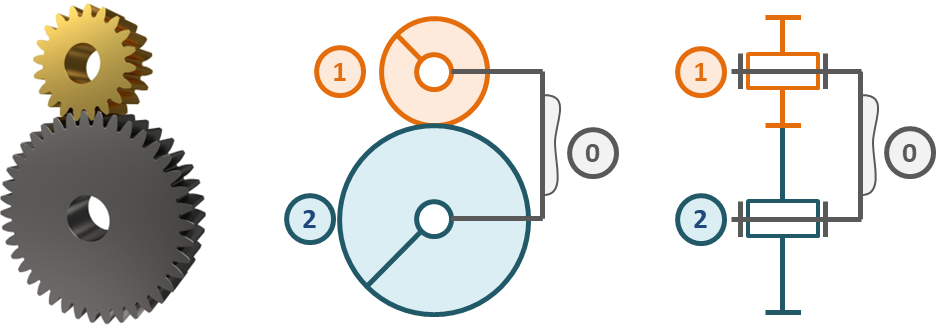
\includegraphics[width=\linewidth]{fig_01.png}
\end{marginfigure}

\section*{Mise en situation}
La mise en mouvement d'une certaine catégorie d'avions de modélisme est assurée par un moteur thermique.   La figure ci-dessous propose un éclaté d'un modèle 3D ainsi que le schéma cinématique associé. 

\begin{marginfigure}
\centering
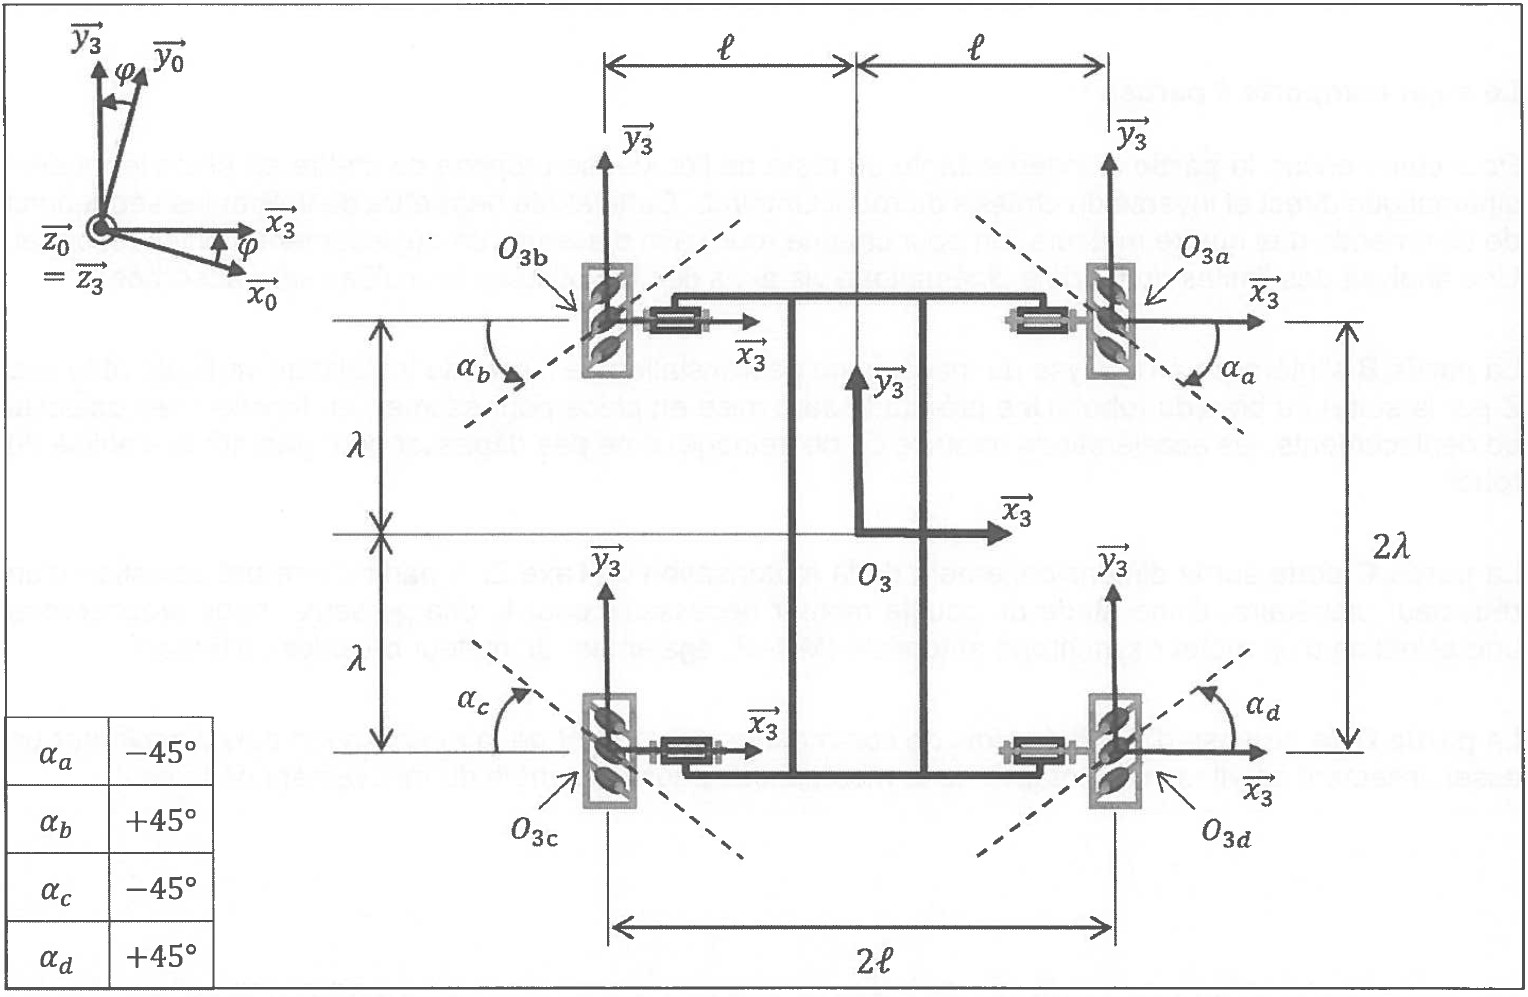
\includegraphics[width=.8\linewidth]{fig_03}
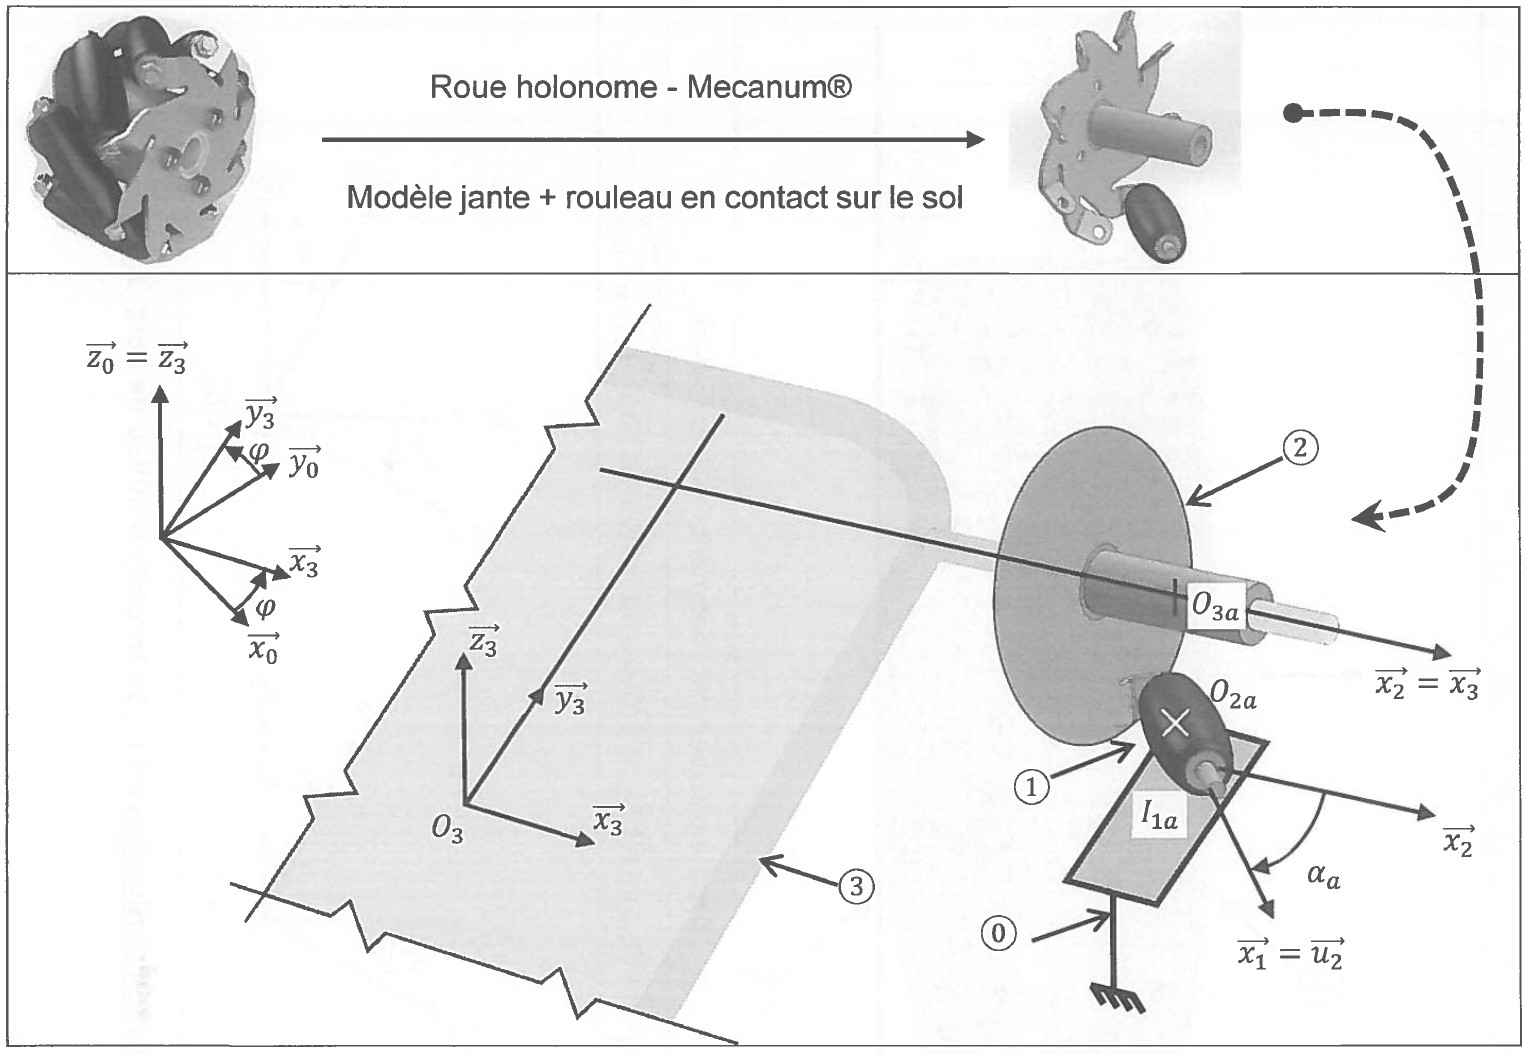
\includegraphics[width=.8\linewidth]{fig_04}
\end{marginfigure}

On appelle : 
\begin{itemize}
\item \textbf{(0)} la bâti lié à la voilure de l'avion;
\item \textbf{(1)} le vilebrequin, solidaire de l'hélice de l'avion;
\item \textbf{(2)} la bielle;
\item \textbf{(3)} le piston.
\end{itemize}

\begin{obj}
\begin{itemize}
\item Déterminer la loi de position et de vitesse du piston pour avoir un taux de rotation du moteur de \SI{9000}{tr.min^{-1}}.
\item Vérifier que l'accélération est inférieure à \SI{10000}{m.s^{-2}}.
\end{itemize}
\end{obj}


\section*{Modélisation}
La modélisation par schéma cinématique est donnée dans le schéma ci-dessous. 
\begin{center}
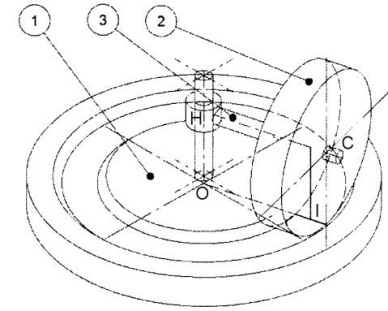
\includegraphics[width=.8\linewidth]{fig_06}
\end{center}
On appelle : 
\begin{itemize}
\item $\mathcal{R}_0=\left(A,\vect{x_0},\vect{y_0},\vect{z_0} \right)$ le repère lié au bâti \textbf{(0)};
\item $\mathcal{R}_1=\left(A,\vect{x_1},\vect{y_1},\vect{z_0} \right)$ le repère lié au vilebrequin \textbf{(1)} avec $\alpha(t)=\left(\vect{x_0},\vect{x_1}\right)$;
\item $\mathcal{R}_2=\left(B,\vect{x_2},\vect{y_2},\vect{z_0} \right)$ le repère lié à la bielle \textbf{(2)} avec $\beta(t)=\left(\vect{x_1},\vect{x_2}\right)$ avec $\vect{AB}\cdot \vect{x_1}=e$ et $e=\SI{5,25}{mm}$;
\item $\mathcal{R}_3=\left(C,\vect{x_3},\vect{y_3},\vect{z_0} \right)$ le repère lié au piston \textbf{(3)} avec $\gamma(t)=\left(\vect{x_2},\vect{x_3}\right)$ avec $\vect{BC}=L\vect{x_2}$ et $\vect{AC}\cdot \vect{y_0}=\lambda(t)$ et $L=\SI{23,9}{mm}$.
\end{itemize}
Les figures planes de changement de repère sont données ci-dessous : 
\begin{center}
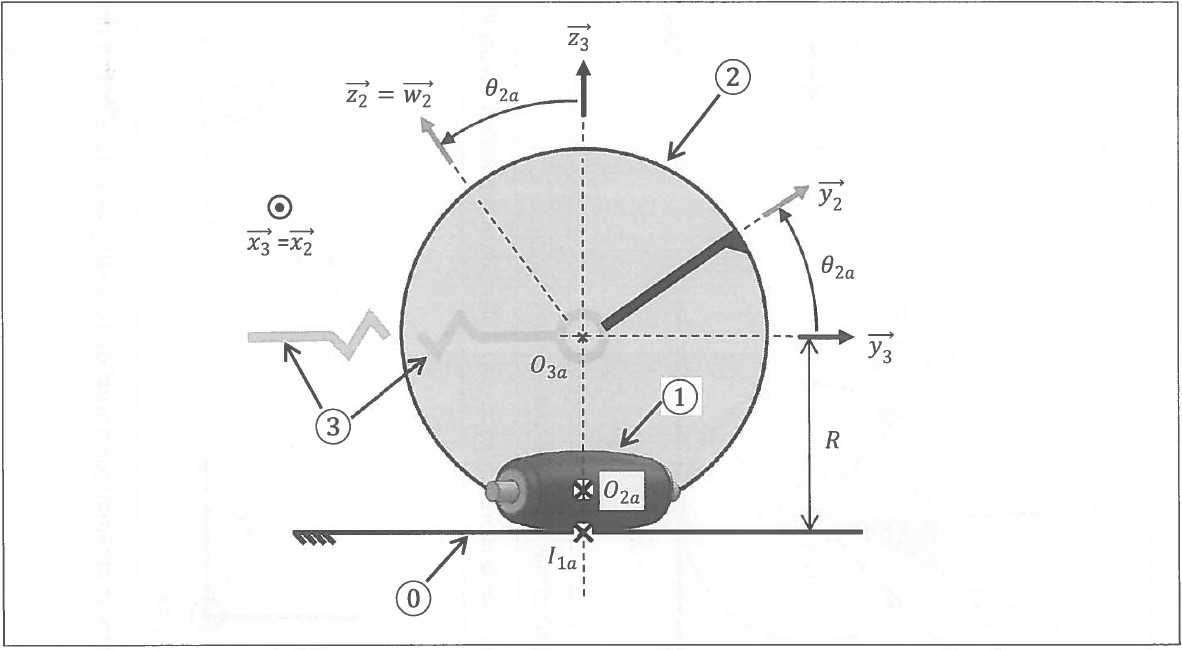
\includegraphics[width=\linewidth]{fig_05}
\end{center}

\question{Tracer le graphe de structure. Définir le nombre de cycles, la mobilité du mécanisme et le nombre de degrés de liberté de chacune des liaisons en 2D et en 3D.}


\question{Préciser la variable d'entrée ainsi que la variable de sortie du système.}

\question{Déterminer la loi entrée-sortie géométrique du système.}
\ifprof 
\begin{corrige} 

Dans le cas d'un système bielle-manivelle comme le moteur de modélisme, on veut connaître la vitesse de rotation de l'hélice $\dot{\alpha}(t)$ en fonction de la vitesse de translation du piston $\dot{\lambda}(t)$. 

La fermeture géométrique est donc la suivante : 
$$\vect{AB} + \vect{BC} +\vect{CD} = \vect{0}.$$

%\Longleftrightarrow d\vect{x_1} + e \vect{x_2} - \lambda(t) \vect{y_0}  = \vect{0}
%\end{eqnarray*}
Le mécanisme étant plan dans le plan $\left(\vect{x_0},\vect{y_0}\right)$, on ne tient pas compte des distances suivant $\vect{z_0}$ et on a : 
$$e\vect{x_1}+L\vect{x_2}-\lambda(t)\vect{y_0}= \vect{0}.$$



Exprimons $\vect{x_1}$ et $\vect{x_2}$ dans la base $\mathcal{R}_0$ :
$$
\left\{
\begin{array}{lcl}
\vect{x_1} & = & \cos \alpha(t) \vect{x_0} + \sin \alpha(t) \vect{y_0} \\
\vect{x_2} & = & \cos \beta(t) \vect{x_1} + \sin \beta(t) \vect{y_1} \\
 & = & \cos \beta(t) \left( \cos \alpha(t) \vect{x_0} + \sin \alpha(t) \vect{y_0} \right) + 
\sin \beta(t) \left( \cos \alpha(t) \vect{y_0} - \sin \alpha(t) \vect{x_0} \right) \\
\end{array}
\right.
$$

On peut aussi observer que directement 
$\vect{x_2} =\cos\left(\alpha(t)+\beta(t) \right)\vect{x_0} + \sin\left(\alpha(t)+\beta(t) \right)\vect{y_0}$.

En projetant l'équation vectorielle sur $\vect{x_0}$ et $\vect{y_0}$ on a : 
$$
%\left\{
%\begin{array}{l}
%d\cos\alpha + e \cos\beta \cos\alpha - e \sin\beta \sin\alpha = 0 \\
%d\sin\alpha +  e \cos\beta \sin\alpha + e \sin\beta \cos\alpha- \lambda= 0 \\
%\end{array}
%\right.
%\Longleftrightarrow 
\left\{
\begin{array}{l}
e\cos\alpha+ L \cos\left(\alpha+\beta\right)  = 0 \\
e\sin\alpha +  L \sin\left(\alpha+\beta \right) - \lambda= 0 \\
\end{array}
\right.
$$

On cherche à éliminer à $\alpha+\beta$ :
$$
\left\{
\begin{array}{l}
L\cos\left(\alpha+\beta\right)  = - e\cos\alpha \\
L \sin\left(\alpha+\beta\right) =  \lambda - e\sin\alpha
\end{array}
\right.
$$

En passant au carré et en sommant les deux expressions, on a donc : 
$$
L^2=e^2\cos^2\alpha + \lambda^2 + e^2\sin^2\alpha-2\lambda e \sin\alpha
=e^2+ \lambda^2 -2\lambda e \sin\alpha.
$$

Et donc :
$$
 \lambda^2 -2\lambda e \sin\alpha+e^2-L^2=0
$$


On a $\Delta = 4e^2\sin^2\alpha - 4\left(e^2 - L^2 \right)$ et 
$\lambda 
= \dfrac{2 e \sin\alpha\pm \sqrt{4e^2\sin^2\alpha - 4\left(e^2 - L^2 \right)}}{2}
=  e \sin\alpha\pm \sqrt{e^2\sin^2\alpha - \left(e^2 - L^2 \right)}$.

Au final, 
$$\lambda(t)=  e \sin\alpha(t)+ \sqrt{e^2\sin^2\alpha(t) - \left(e^2 - L^2 \right)}$$
%Pour exprimer $\lambda$ en fonction de $\alpha$, il faut donc résoudre une équation du second degré. Pour exprimer $\alpha$ en fonction de $\lambda$, la méthode est directe. 


%Résolvons donc 
%$$
%\lambda^2 +2d\lambda\sin\alpha +d^2- e^2=0
%$$
%On calcule le discriminant :
%$$
%\Delta = 4d^2\sin^2\alpha-4\left( d^2- e^2\right)
%$$

%On a donc 
%$$
%\lambda 
%= \dfrac{-2d\sin\alpha \pm \sqrt{\Delta}}{2}
%= -d\sin\alpha \pm \sqrt{d^2\sin^2\alpha-\left( d^2- e^2\right)}
%$$
\end{corrige}
\else
\fi
\question{Déterminer la loi entrée-sortie cinématique du système.}
\ifprof
\begin{corrige}
Il suffit de dériver l'expression précédente :
$$\lambda(t)=  e \dot{\alpha}(t)\cos\alpha(t)+ \dfrac{1}{2}\left(2e^2\dot{\alpha}(t)\sin\alpha(t)\cos\alpha(t) \right)\left(e^2\sin^2\alpha(t) - \left(e^2 - L^2 \right)\right)^{-\dfrac{1}{2}}.$$
\end{corrige}
\else
\fi

\question{Tracer l'allure de la loi de vitesse du piston.}
\ifprof
\begin{corrige}
\begin{center}
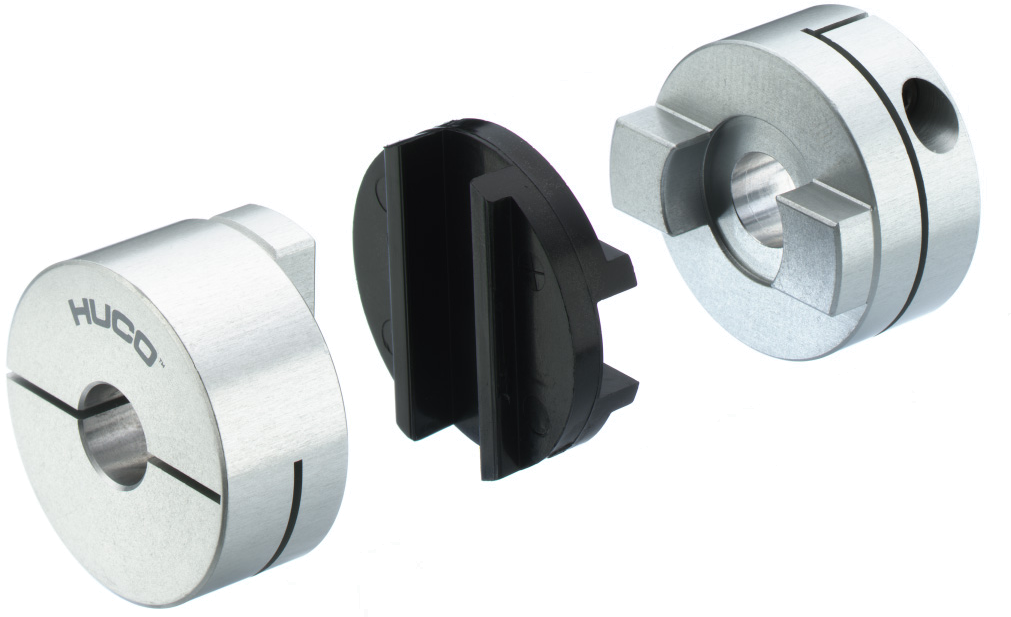
\includegraphics[width=\linewidth]{fig_08}
\end{center}
\end{corrige}
\else
\fi


Une simulation réalisée sous Méca3D permet d'obtenir l'évolution de l'accélération du piston : 

\begin{center}
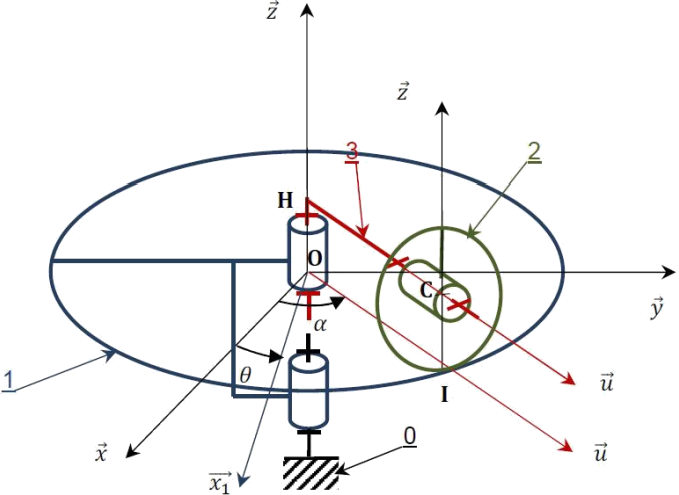
\includegraphics[width=.7\linewidth]{fig_07}
\end{center}


\question{Conclure vis-à-vis du cahier des charges.}

